\chapter{Introduction}\label{ch:introduction}

% Goals:
% - contextualize RC in physics
% - new field, interest, ML physics
% - outline rest, put important figures in intro
% - who helped and what did I do

Recently, many difficult problems have been solved using methods from
the field of machine learning, in particular using neural
networks. Machine learning methods work by learning solutions from
example data alone, without the need for an existing model for that
data.  Physicists have used neural networks to find the masses of
particles from decay data~\cite{lonnblad1992} and separate quark and
gluon jets in $e^+ e^-$ annihilation~\cite{csabai1991}.  In other
fields, this approach has been used effectively on handwritten digit
recognition~\cite{lecun1998,simard2003}, speech
recognition~\cite{hinton2012}, and speech production~\cite{oord2016}.
These are all problems with large sets of example data, but which are
otherwise difficult or intractable with a more traditional programming
approach. Put simply, it is easy to provide examples of what the
number ``\num{2}'' looks like, while it is difficult to define what
features a written ``\num{2}'' must have in a programming language.

By its nature, many problems in physics are defined in terms of
time-varying data. Neural networks that contain internal cycles,
called recurrent neural networks, are a natural fit for these
problems. The addition of cycles gives the resulting network memory
and allows it to be used to effectively solve many time-domain
problems, such as forecasting chaotic
systems~\cite{garcia-pedrero2010}. However, this modification has a
cost: recurrent neural networks take much more time to train, as the
training algorithm takes exponentially longer to learn how to utilize
past inputs~\cite{bengio1994,lukosevicius2009}.

More recently, a new machine learning tool has emerged for dealing
with time-domain problems.  Known as \emph{reservoir computing}, this
tool was originally formulated as a novel way to reduce the
computational cost of training recurrent neural
networks~\cite{lukosevicius2009}. Reservoir computers (RCs) have been
effectively applied to chaotic system
forecasting~\cite{jaeger1978,pathak2017} and system state
inference~\cite{lu2017}. More than just short-term prediction, RCs are
capable of reproducing the \emph{climate} of a dynamical
system~\cite{pathak2017,haluszczynski2019}, that is, it learns the long-term
features of the system such as the system's attractor and Lyapunov
exponents.

RCs are interesting to physicists not only as a tool to solve
problems. At the heart of a RC is a dynamic system called the
\emph{reservoir}, which provides the rich dynamics the RC draws on to
function. This is usually implemented as a neural network, but in
practice many dynamic systems function well. This opens the door to
building RCs around real physical systems, such as a network of
autonomous logic on an FPGA~\cite{canaday2018} or an optical feedback
system~\cite{antonik2016}. This is interesting from a theoretical
perspective, as physical RCs use an ancillary system to help answer
questions about a main system, but they are also practically
interesting: by relying on physical reservoirs, rather than
simulation, these methods perform chaotic system forecasting and other
tasks at a very high rate.

As a new field, reservoir computing still has many unanswered
fundamental questions. What qualities should the internal reservoir
have to create a good RC? A common practice is to use a random network
as the reservoir, generated from a set of meta-parameters. There are a
handful of heuristics for some parameters, such as setting the
\emph{spectral radius} of the network near one and the need for
recurrent network connections~\cite{jaeger2001,lukosevicius2012}, but
the applicability of these rules is narrow. What features of the
reservoir are necessary, and which can be discarded?

In this dissertation, I construct reservoir computers that do not
follow the conventional rules for reservoir construction. These RCs
continue to perform well on chaotic system forecasting and state
inference, and can even reproduce the chaotic attractor of the system
they have learned, despite the fact that their internal reservoir has
no recurrent connections. Indeed, by the end of this dissertation, they do
not have an internal reservoir at all.

\section{Outline and Summary of Contributions}

In this dissertation, \cref{ch:reservoir-computing,ch:nvar} provide
background information on the methods used, while
\cref{ch:low-connectivity,ch:nvar-application} present new
contributions. These contributions are summarized in \cref{tab:contribution}.

\begin{figure}
  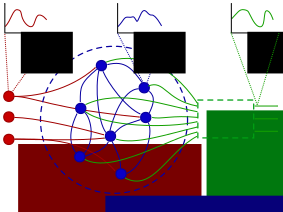
\includegraphics[width=0.6\textwidth]{figures/reservoir}
  \caption{High-level view of an echo state network RC.  An input
    signal (red, top left) drives an internal reservoir to produce a
    reservoir response (blue, top center) which is then combined to
    form an output signal (green, top right). In an ESN, the reservoir
    network has external input signals (red nodes, left) that drive
    the internal network (blue nodes, center) to produces an overall
    output (green, right).  Each internal node may have two kinds of
    input connections: connections to other nodes in the network
    ($W_r$, blue arrows), or connections to the overall input
    ($W_\text{in}$, red arrows). Each node may also contribute to the
    overall output ($W_\text{out}$, green arrows). Note that the
    internal connections may contain cycles.  When the ESN is used to
    perform forecasting, the output on the right side is connected to
    the input on the left side, allowing the ESN to run autonomously
    with no external input.}%
  \label{fig:intro-reservoir}
\end{figure}

In \cref{ch:reservoir-computing}, I describe the reservoir computing
method, as well as a common concrete implementation of a RC called an
\emph{echo state network} (ESN) summarized in \cref{fig:intro-reservoir}. I
explain how to construct an ESN, the meta-parameters that govern its
construction, and discuss some of the limited known results for
choosing these meta-parameters. Then, I discuss how the RC is trained,
both for autonomous forecasting tasks and for inference tasks, as well
as how performance quality on these tasks is commonly measured. I
briefly discuss the known problems with this performance measure, and
suggest a new measure designed to mitigate these problems.

\begin{table}
  \caption{A summary of chapters and associated contributions.}
  \begin{tabularx}{\linewidth}{llcX}
    & Chapter & & Contribution \\
    \hline
    \rule{0pt}{4ex}%
    & \Cref{ch:reservoir-computing} & $\bullet$ & introduce a new metric $\tilde{\epsilon}$ \\
    & \nameref{ch:reservoir-computing} & & \\
    \rule{0pt}{4ex}%
    \cite{griffith2019}
    & \Cref{ch:low-connectivity} & $\bullet$ & demonstrate new metric $\tilde{\epsilon}$ \\
    & \nameref{ch:low-connectivity} & $\bullet$ & explore ESNs with very low connectivity \\
    & & $\bullet$ & demonstrate these ESNs perform equally well as traditional ESNs \\
    \rule{0pt}{4ex}%
    \cite{gauthier2021}
    & \Cref{ch:nvar-application} & $\bullet$ & demonstrate NVARs on forecasting/inference \\
    & \nameref{ch:nvar-application} & $\bullet$ & show that NVARs perform as well as ESNs even with a low number of taps \\
    & & $\bullet$ & use RC-style linear regression to improve NVAR generalization \\
    & & $\bullet$ & explore current limitations of NVAR approach \\
  \end{tabularx}
  \label{tab:contribution}
\end{table}

\begin{figure}
  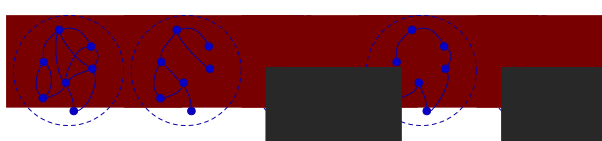
\includegraphics[width=0.7\textwidth]{figures/topology}
  \caption{The five reservoir structures tested. Only internal
    reservoir connections are pictured. Connections to the reservoir
    computer input, or to the output layer are not shown. (a) A
    general, fixed in-degree network, here pictured with $N=7$ and
    $k=2$. (b) A $k=1$ network with a single connected component. (c)
    A $k=1$ network with the single cycle cut at an arbitrary
    point. (d) A \emph{simple cycle reservoir}. (e) A \emph{delay line
      reservoir}.}%
  \label{fig:intro-topology}
\end{figure}

In \cref{ch:low-connectivity}, I apply ESNs to the task of chaotic
system forecasting for three different chaotic systems, using my new
metric. I demonstrate that this new metric more accurately reflects
some long-term forecasting failures that the traditional metric does
not. I use a Bayesian optimization algorithm to tune the
meta-parameters for the ESNs, and in so doing, discover a class of
well-performing ESNs with very simple internal reservoirs. I identify
four classes of reservoir networks with particularly simple structure,
summarized in \cref{fig:intro-topology}. Of these, two had been
previously identified. I build on this work and demonstrate that all
four classes have the capacity to perform equally well as a traditional
ESN. In particular, all four classes can reproduce the chaotic
attractor of the system they are trained on. I then discuss the
trade-offs between these simpler reservoir structures and a
traditional ESN.

\begin{figure}
  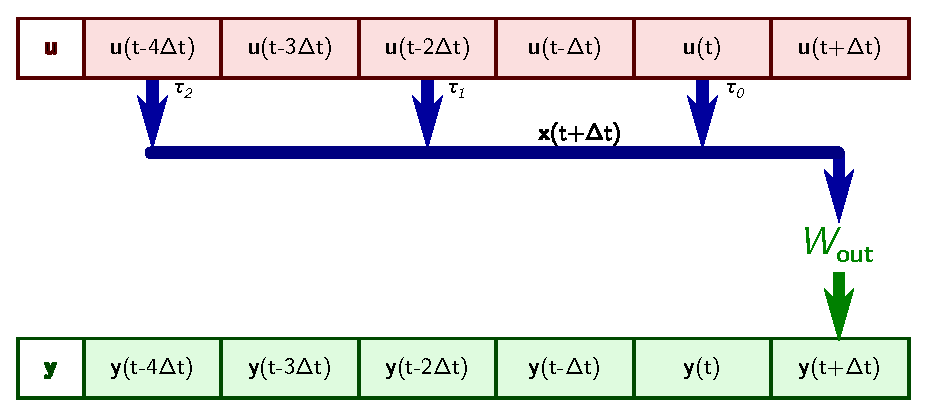
\includegraphics{figures/var-infer}
  \caption{Summary of the (N)VAR method. Many time-delay taps $\tau_i$
    of the discrete-time signal $\bm{u}(t)$ (top, red) are concatenated into the tap
    vector $\bm{v}(t)$ (middle, blue). Here, there are three taps
    $\tau_0=0$, $\tau_1=2$, and $\tau_2=4$. These taps are then passed
    through a possibly nonlinear function $\bm{g}_\text{n}$ and
    combined linearly by the output matrix $W_\text{out}$ to produce
    the next value of the (N)VAR's output $\bm{y}(t)$ (bottom,
    green). For a linear VAR, $\bm{g}_\text{n}$ is the identity
    function. To transform a whole time series input, this (N)VAR process
    slides along the time axis from left to right.}
  \label{fig:intro-var-infer}
\end{figure}

In \cref{ch:nvar}, I describe a different technique known as nonlinear
vector auto-regression (NVAR), which has recently been shown to be
mathematically equivalent to an ESN under certain conditions.  This
technique is summarized in \cref{fig:intro-var-infer}.  I outline this
proof, discuss the construction and training of an NVAR, and describe
how to apply it to common RC tasks. Then, I discuss the parallels
between the NVAR and RC approaches, as well as the practical
considerations of applying this equivalence proof. Finally, I discuss
the trade-offs between the two approaches.

\begin{figure}
  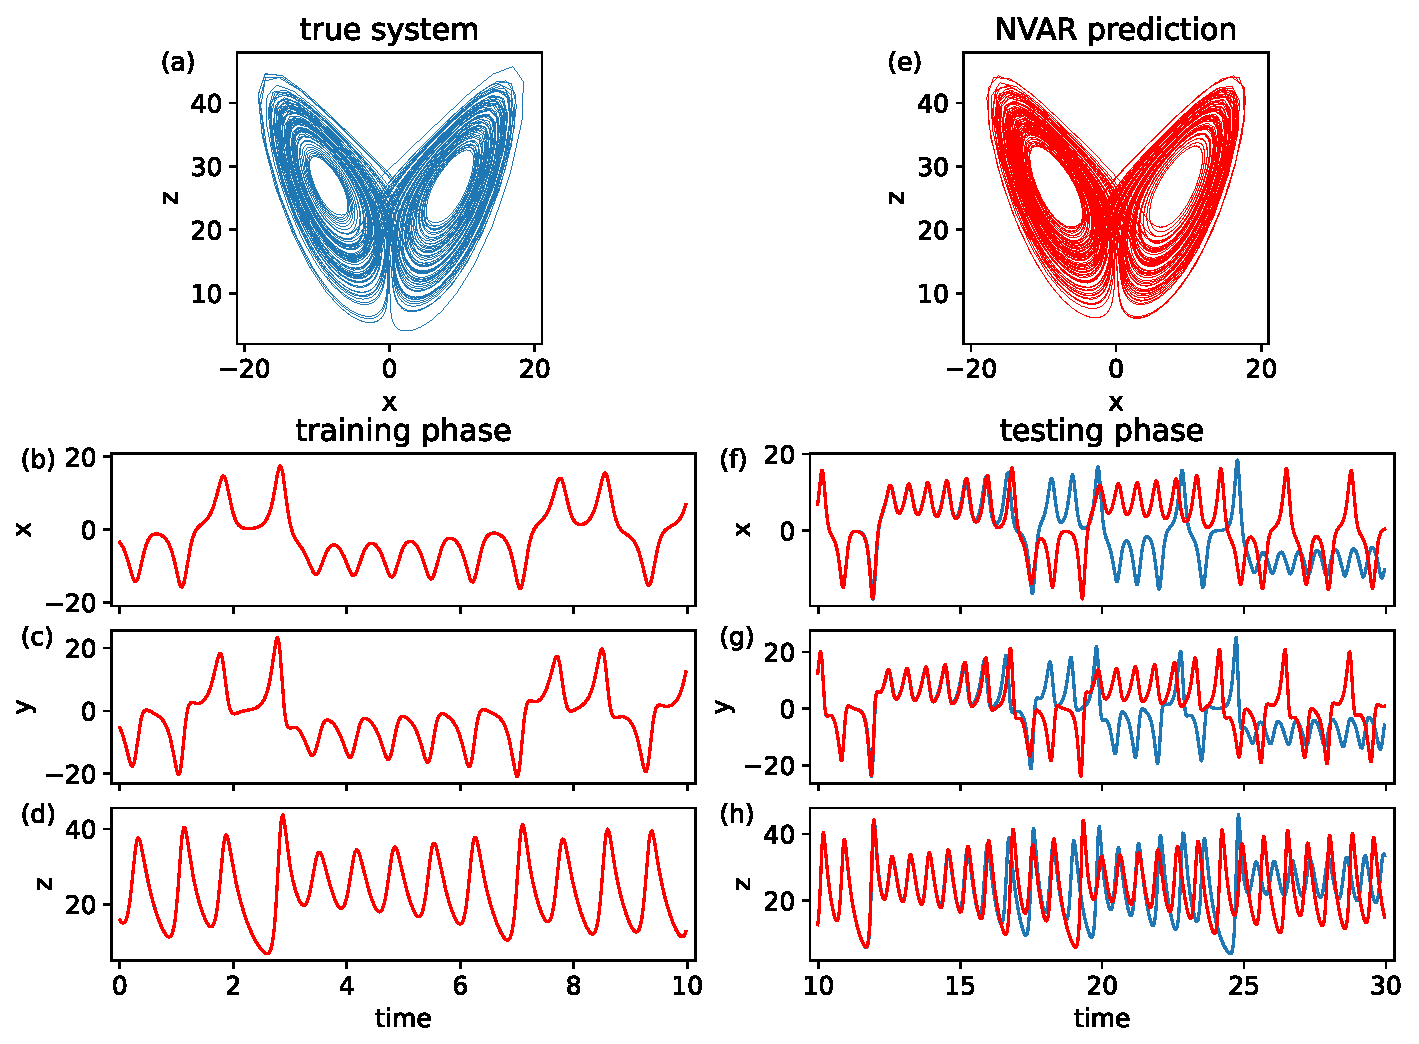
\includegraphics[width=\textwidth]{figures/nvar-predict-lorenz}
  \caption{The true Lorenz attractor (a) and NVAR predicted attractor
    (e) for a single training trial. (b) -- (d) True Lorenz system
    (blue) during training overlaid with NVAR output (red) calculated
    after training is complete. (f) -- (h) True (blue) and NVAR
    forecasted output (red). The NVAR shows good agreement with the
    true system as far as $5$ Lyapunov periods in to the autonomous
    forecast.}
  \label{fig:intro-nvar-predict-lorenz}
\end{figure}

In \cref{ch:nvar-application}, I build on this equivalence with my
collaborators to demonstrate NVARs solving two common RC tasks: system
forecasting (as in \cref{fig:intro-nvar-predict-lorenz}) and state
inference.  I show that NVARs are capable of ESN-equivalent performance
on these tasks even under conditions where the equivalence proof does
not strictly hold. The NVARs achieve this performance despite being
considerably simpler than an ESN and with very little training data and
training time. In addition, I discuss how a trained NVAR can provide
interpretable results, while a trained RC is opaque. I then show how
the NVAR approach can be extended naturally to solve a wider array of
problems. Finally, I discuss how this approach may replace traditional
RCs, and what questions remain to be answered before that can happen.

Finally, in \cref{ch:conclusion}, I summarize my findings and
contributions, and propose interesting new directions for future
research discovered during this work.
